\subsection{Gráfico de Hastes ou Bastões}

O gráfico de hastes ou bastões é muito utilizado para representar dados não agrupados em classes, o que normalmente ocorre com dados discretos. Nesse caso, não há perda de informação pois os valores da variável aparecem individualmente, conforme constam da amostra. Com relação a sua construção, basta representarmos as frequências simples absolutas ou relativas de cada elemento do conjunto de dados.

\begin{figure}[H]
  \centering
  \begin{tikzpicture}
    \begin{axis}[
      xmin=-0.5, xmax=7,
      ymin=0, ymax=30,
      axis x line=middle,
      axis y line=middle,
      width=0.8 \textwidth,
      height=7cm,
      tick align=outside,
      grid=both,
      minor tick num=1,
      xlabel={$x$},
      ylabel={$y$},
      x axis line style={-{Stealth[length=3mm]}},
      y axis line style={-{Stealth[length=3mm]}},
    ]
      \filldraw[thick, fill=gray!30] (axis cs:0,4) circle[radius=1.5mm];
      \filldraw[thick, fill=gray!30] (axis cs:1,10) circle[radius=1.5mm];
      \filldraw[thick, fill=gray!30] (axis cs:2,25) circle[radius=1.5mm];
      \filldraw[thick, fill=gray!30] (axis cs:3,15) circle[radius=1.5mm];
      \filldraw[thick, fill=gray!30] (axis cs:4,10) circle[radius=1.5mm];
      \filldraw[thick, fill=gray!30] (axis cs:5,5) circle[radius=1.5mm];
      \filldraw[thick, fill=gray!30] (axis cs:6,1) circle[radius=1.5mm];
      \draw[blue, ultra thick] (0,0) -- (0,4);
      \draw[blue, ultra thick] (1,0) -- (1,10);
      \draw[blue, ultra thick] (2,0) -- (2,25);
      \draw[blue, ultra thick] (3,0) -- (3,15);
      \draw[blue, ultra thick] (4,0) -- (4,10);
      \draw[blue, ultra thick] (5,0) -- (5,5);
      \draw[blue, ultra thick] (6,0) -- (6,1);
    \end{axis}
  \end{tikzpicture}
  \caption{Gráfico de Hastes}
\end{figure}

O histograma é um gráfico destinado a representar dados agrupados em classe, sendo composto por um conjunto de retângulos contíguos (justapostos) cujas bases ficam localizadas sobre o eixo horizontal (eixo x), de forma que os seus pontos médios devem coincidir com os pontos médios dos intervalos de classe e seus limites devem coincidir com os limites da classe.

A quantidade de retângulos em um histograma é equivalente ao número de intervalos de classe. A largura de cada retângulo deve ser igual à amplitude do intervalo de classe, enquanto a altura precisa ser proporcional à frequência do intervalo de classe. Além disso, a área do histograma é proporcional ao somatório das frequências.

\begin{figure}[ht]
\centering
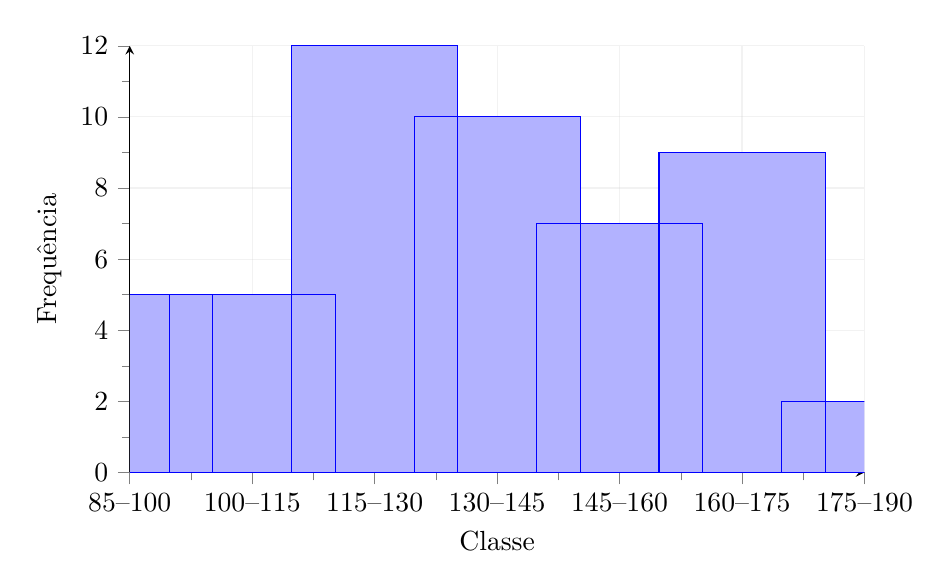
\begin{tikzpicture}
\begin{axis}[
  ybar,
  ymin=0,
  width=0.9\textwidth,
  height=7cm,
  axis lines=left,
  tick align=outside,
  grid=major,
  minor tick num=1,
  major grid style={opacity=0.2},
  xlabel={Classe},
  ylabel={Frequência},
  symbolic x coords={{85--100},{100--115},{115--130},{130--145},{145--160},{160--175},{175--190}},
  xtick=data,
  bar width=60pt,
  enlarge x limits=0
]
\addplot coordinates {
  ({85--100}, 5)
  ({100--115}, 5)
  ({115--130}, 12)
  ({130--145}, 10)
  ({145--160}, 7)
  ({160--175}, 9)
  ({175--190}, 2)
};
\end{axis}
\end{tikzpicture}
\caption{Histograma (classes e frequências).}
\end{figure}
A diferença básica entre um histograma e um gráfico de colunas (estudaremos na próxima seção) é a separação entre os retângulos adjacentes. Veja que não existe separação entre os retângulos no caso do histograma.

Dito isso, é importante mencionarmos a existência do gráfico denominado de poligonal
característica, que construímos utilizando somente os contornos do histograma.
\begin{figure}[hbt]
  \centering
  \begin{tikzpicture}
    \begin{axis}[
    xmin=80, xmax=200,
    ymin=0, ymax=14,
    axis x line=middle,
    axis y line=middle,
    width=0.8 \textwidth,
    height=7cm,
    %scale only axis,
    %scaled y ticks=true,
    %ytick scale label code/.code={$\times 10^{#1}$},
    %xtick distance=10, % ajuste: 5, 10, 20...
     x axis line style={-{Stealth[length=3mm]}},
     y axis line style={-{Stealth[length=3mm]}},
      tick align=outside,
      grid=major,
      minor tick num=1,
      xlabel={$x$},
      ylabel={$y$},
    ]
           \addplot[
        thick, red
      ] coordinates {
        (85,0)
        (85,5)
        (115,5)
        (115,12)
        (130,12)
        (130,10)
        (145,10)
        (145,7)
        (160,7)
        (175,7)
        (175,9)
        (190,9)
        (190,2  )
      };
    \end{axis}
  \end{tikzpicture}
  \caption{Contorno do Histograma.}
\end{figure}

\subsection{Polígono de Frequências}

    O polígono de frequências é um gráfico em linha obtido por meio da ligação, por segmentos de reta, dos pontos médios das bases superiores dos retângulos de um histograma. Também é necessário considerar a existência de uma classe anterior à primeira e outra posterior à última, ambas com a frequência nula.

    \begin{figure}[H]
        \centering
            \includegraphics[width=0.6 \linewidth]{histograma_poligono.png}
            \caption{Histograma com polígono}
        \end{figure}

\subsection{curva de Frequências}
A curva de frequências é obtida a partir do polimento de um polígono de frequências. Em sentido geométrico, o polimento corresponde à eliminação dos vértices (cantos) da linha poligonal. Esse processo suaviza os contornos do polígono de frequências, o que evidencia a verdadeira natureza dos dados em análise.

O polígono de frequências fornece a imagem real do fenômeno investigado, enquanto a curva de frequência mostra sua tendência. Naturalmente, quando o conjunto de dados é grande, a linha poligonal se torna curva. Por isso, podemos afirmar que a curva de frequência antecipa o comportamento da distribuição para um número maior de dados.

O processo de polimento é realizado por meio da seguinte fórmula:
\medskip
\[
    fc_i=\frac{f{ant}+2\times f_i+f_{post}}{4}
\]
\medskip
\begin{table}
    \centering
    \begin{tabular}{lccc}
        \toprule
        \shortstack{Tempo \\Médio\\\((X_i)\)}&\shortstack{Ponto \\Médio\\\((PM_i)\)} &Frequência\((f_i)\)&\shortstack{Frequência \\Calculada}\\
            \midrule
        \(70\leq\,x\,<85\)    &77,5   &0  &\(fc_0=\frac{0+2\times 0+5}{4}=1,25\)\\
        \(85\leq\,x\,<100\)   &92,2   &5  &\(fc_1=\frac{0+2\times 0+5}{4}=3,75\)\\
        \(100\leq\,x\,<115\)  &107,5  &5  &\(fc_2=\frac{0+2\times 0+5}{4}=6,75\)\\
        \(115\leq\,x\,<130\)  &122,5  &12 &\(fc_3=\frac{0+2\times 0+5}{4}=9,75\)\\
        \(130\leq\,x\,<145\)  &137,5  &10 &\(fc_4=\frac{0+2\times 0+5}{4}=9,75\)\\
        \(145\leq\,x\,<160\)  &152,5  &7  &\(fc_5=\frac{0+2\times 0+5}{4}=8,75\)\\
        \(160\leq\,x\,<175\)  &167,5  &9  &\(fc_6=\frac{0+2\times 0+5}{4}=6,75\)\\
        \(175\leq\,x\,<190\)  &192,5  &2  &\(fc_7=\frac{0+2\times 0+5}{4}=3,25\)\\
        \(190\leq\,x\,<205\)  &197,5  &0  &\(fc_8=\frac{0+2\times 0+5}{4}=0,50\)\\
        \bottomrule
    \end{tabular}
    \caption{Frequências calculadas}
\end{table}

\begin{figure}[H]
  \centering
  \includegraphics[width=0.8 \linewidth]{curva_de_frequencia.png}
  \caption{Curva de Frequência}
\end{figure}